\chapter{LHC-ATLAS実験}
\label{chapter2}

LHC-ATLAS 実験とは、Large Hadron Collider (LHC) を用いた高エネルギーの陽子–陽子衝突によって生成された粒子を ATLAS (A Troidal LHC ApparatuS) 検出器によって検出し、標準模型の精密測定や新粒子探索などを行う実験である。
LHC は 2018 年に Run-2 を終了し、2019 年から 2021 年にかけて LHC 及び ATLAS 検出器のアップグレードが行われ、2022 年からは Run-3 として運転を再開している。

本章では、Run-3 における LHC 及び ATLAS 検出器の概要と ATLAS 実験で採用されているトリガーシステムについて述べる。

\section{LHC加速器}
\label{section2-1}
Large Hadron Collider (LHC)は、スイスのジュネーブ郊外にある欧州素粒子原子核研究機構 (CERN) の地下に建設された周長約 27 km の世界最大の大型ハドロン衝突型加速器である。LHC の全体像を図\ref{fig:LHC_overview}に示す。
LHC は重心系エネルギー 14 TeV、瞬間ルミノシティ $1.0\times10^{34}$ cm$^{-2}$s${^-1}$ で陽子-陽子衝突が可能なように設計されている。

\begin{figure}[tb]
  \centering
  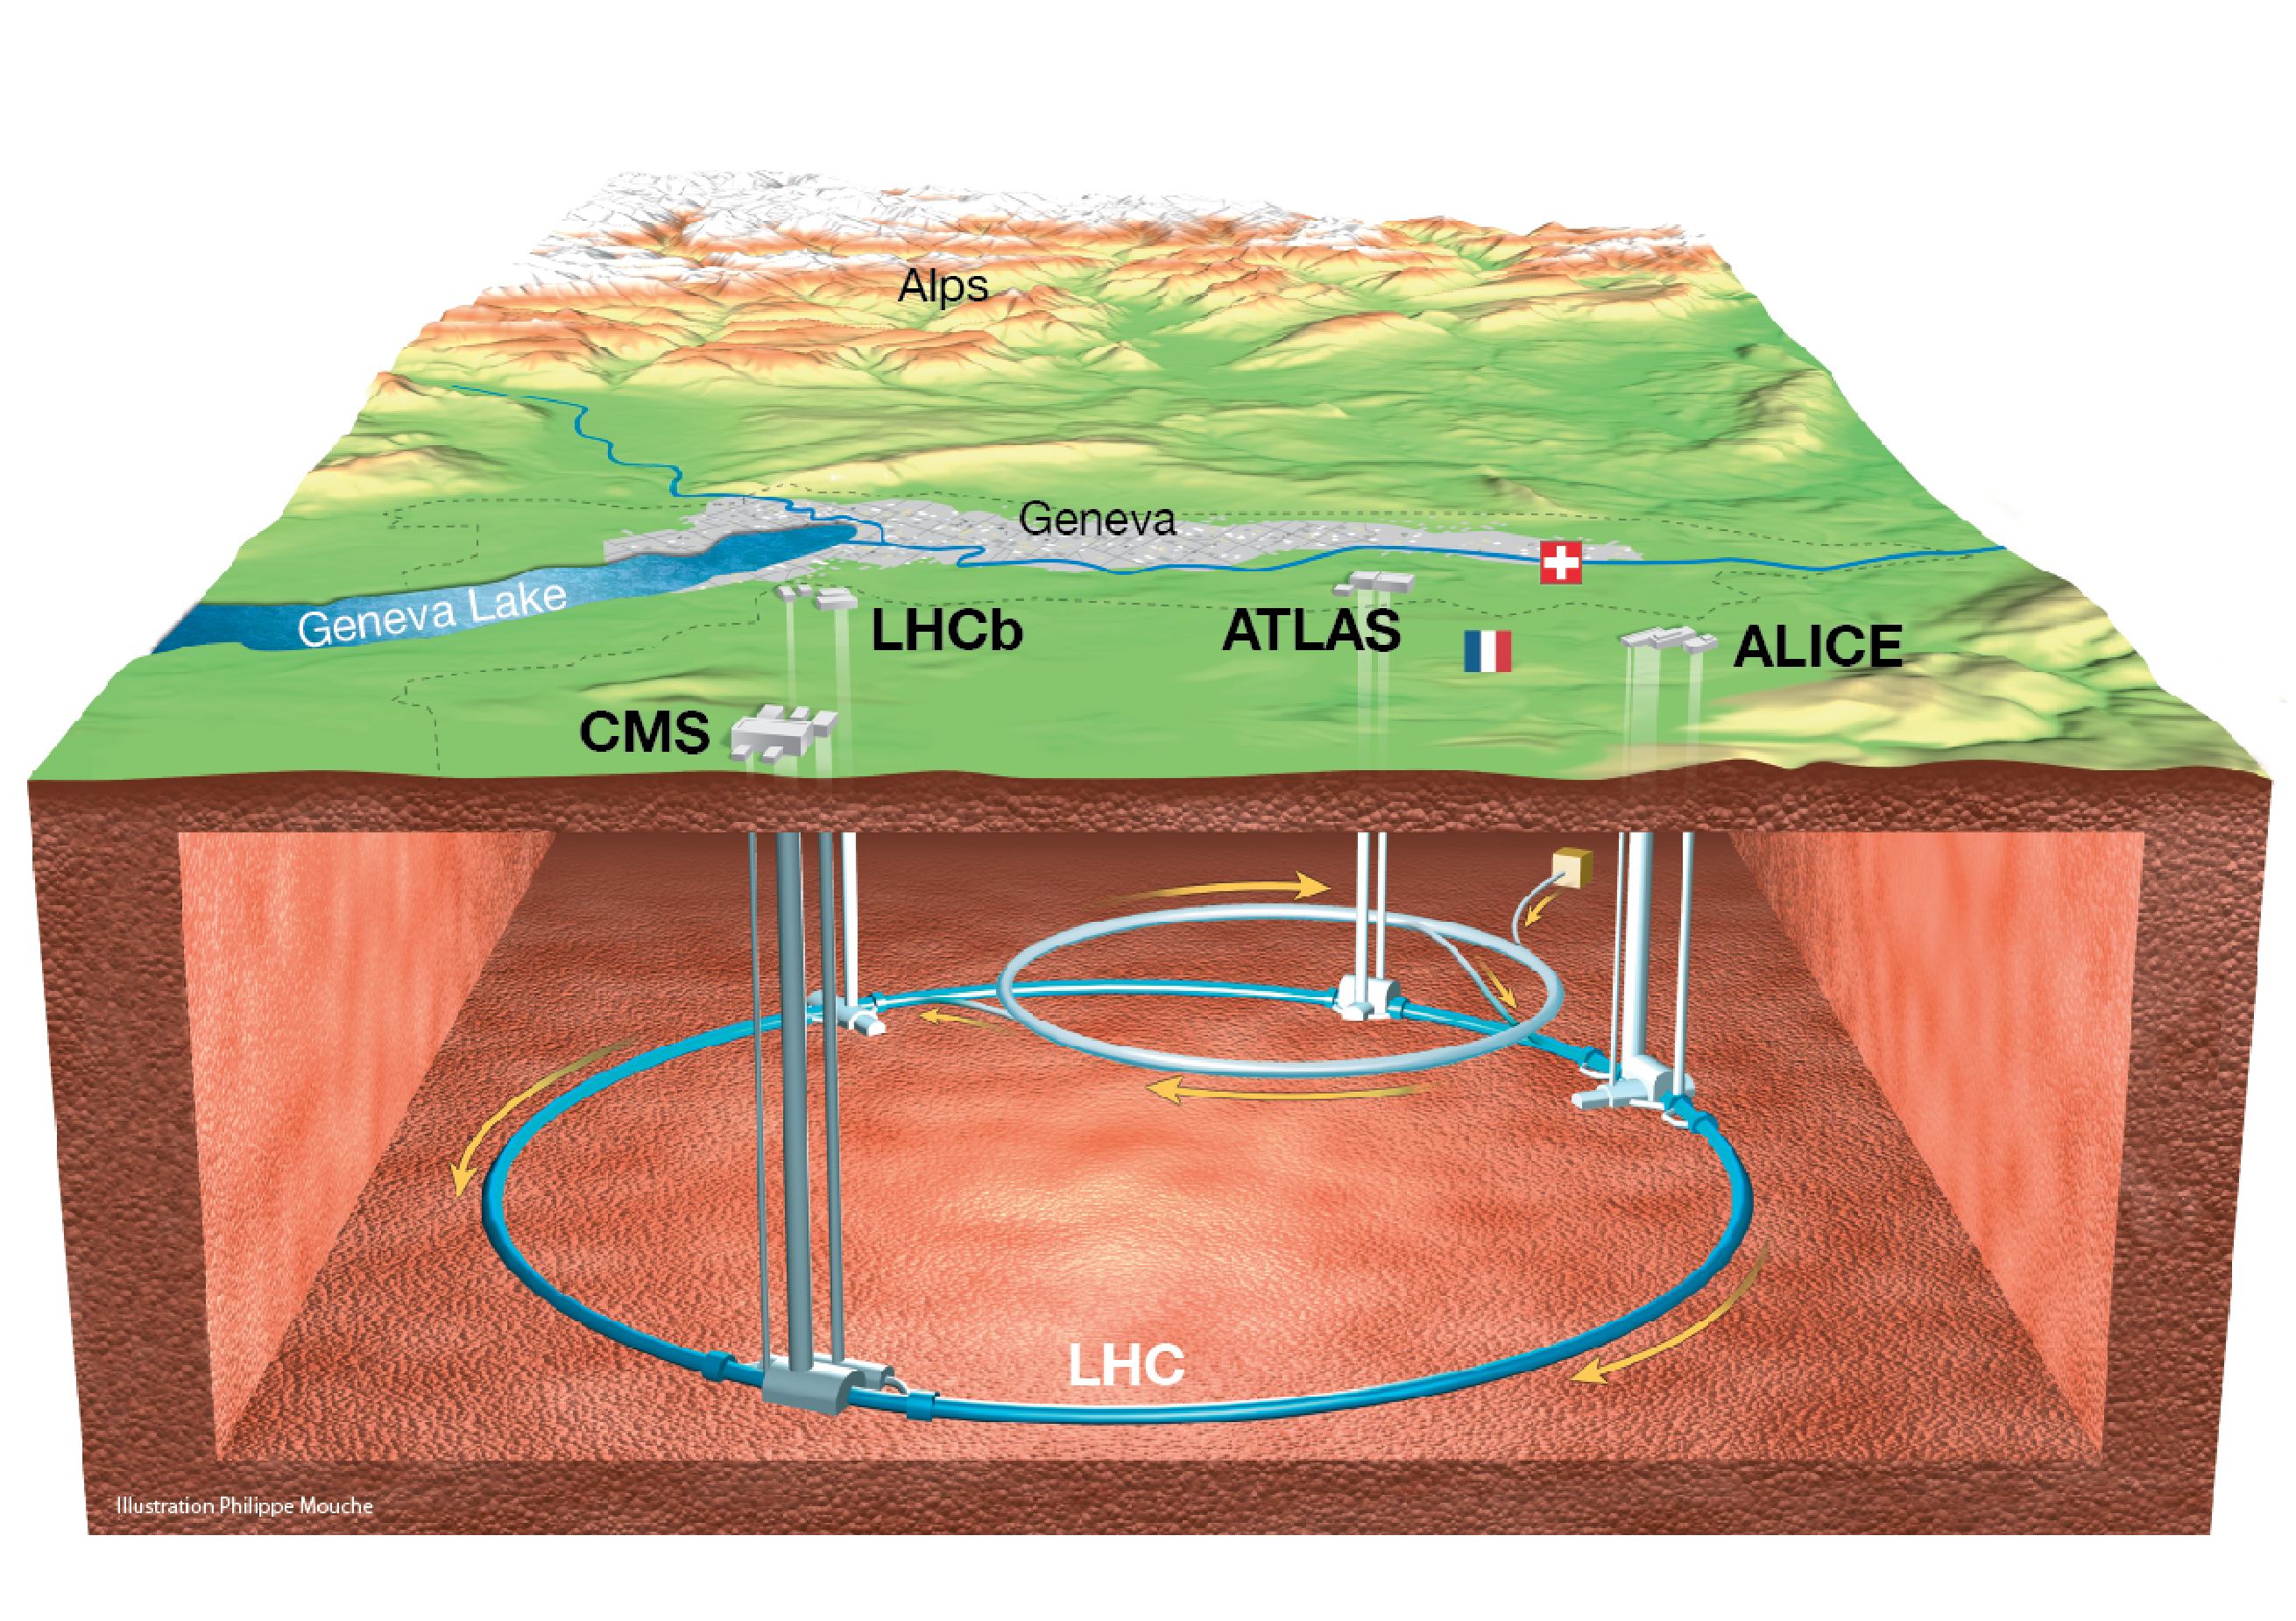
\includegraphics[clip, width=14cm]{fig/2/LHC_overview.pdf}
  \caption{LHC加速器の全体図。}
  \label{fig:LHC_overview}
\end{figure}

\begin{figure}[tb]
  \centering
  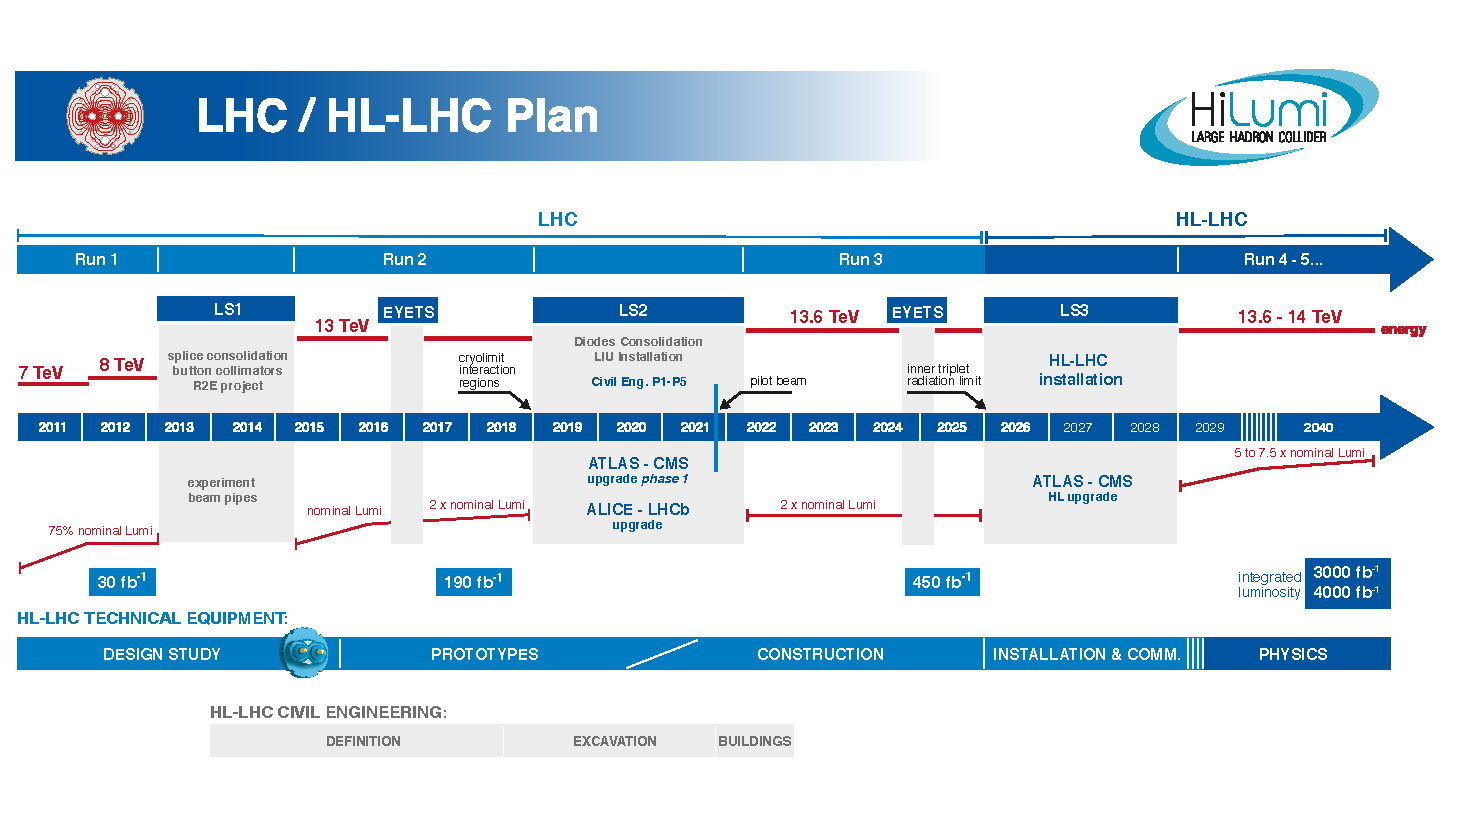
\includegraphics[clip, width=14cm]{fig/1/HL-LHC_Janvier2022.pdf}
  \caption{LHC 加速器の運転とアップグレード計画。LHC では2019年から2022年初旬までの間に Phase-1 Upgrade が行われ、現在は Run-3 として運転を再開している。}
  \label{fig:LHC_Plan}
\end{figure}

LHC は2010年から本格的に実験を開始し、2010年から2012年にかけて行われた運転を Run-1、2015年から2018年にかけて行われた運転を Run-2と呼ぶ。図\ref{fig:LHC_Plan}に LHC 加速器の運転計画を示す。
Run-1 では重心系エネルギー7-8 TeV、瞬間最高ルミノシティ$0.77\times10^{34}$ cm$^{-2}$s${^-1}$での運転を行い、Run-2 では重心系エネルギー13 TeV、瞬間最高ルミノシティ$2.0\times10^{34}$ cm$^{-2}$s${^-1}$での運転を行った。
2019年から2021年初旬までに期間に加速器のアップグレードが行われ、2022年初旬から2025年にかけて行われる Run-3 では陽子-陽子衝突の重心系エネルギーを 13.6 TeV、瞬間ルミノシティ 2.0$\times$10$^{34}$ cm$^{−2}$s$^{−1}$ での運転を行い、Run-2 で取得したデータと合わせて積分ルミノシティ 350 fb$^{−1}$ のデータを取得する予定である。

\begin{figure}[tb]
  \centering
  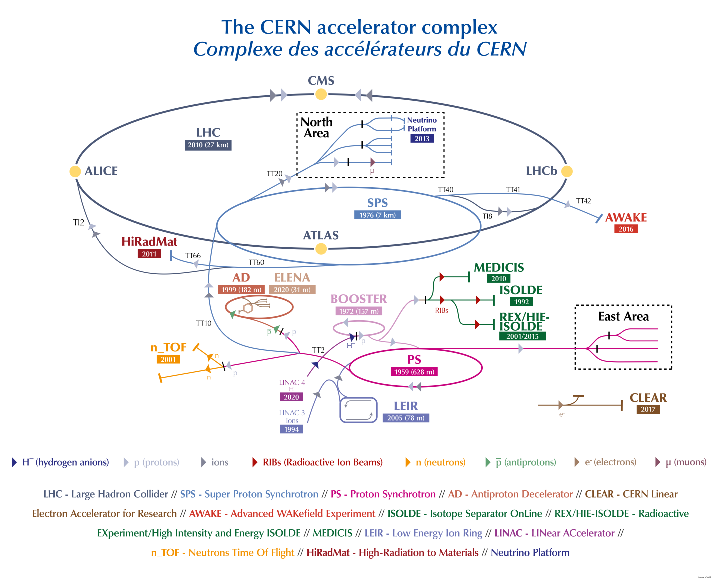
\includegraphics[clip, width=14cm]{fig/2/CCC-v2022.pdf}
  \caption{CERN に設置されている加速器群。}
  \label{fig:LHC加速器}
\end{figure}


LHCでは陽子を衝突させるまでに、いくつかの前段加速器を使用し TeV スケールのエネルギーまで陽子を加速している。図\ref{fig:LHC加速器}に概略図を示す。
初めに負水素イオン(H-、水素原子に電子を加えたもの)を線形加速器である LINAC4 で 160 MeV まで加速する。次に、強い電場をかけることで負水素イオンから2 個の電子を剥ぎ取り、陽子だけの状態にする。そして、Proton Synchrotron Booster (PSB) に入射し 1.4 GeVまで加速された後、Proton Synchrotron (PS) で陽子を26GeVまで加速し、40 MHzのバンチ構造を持った陽子ビームを形成する。
その後、Super Proton Synchrotron (SPS) で450 GeVまで加速された後、陽子ビームは LHC に入射され最大で7 TeV まで加速される。
LHCの衝突実験で使用される陽子ビームはバンチと呼ばれる 10${^11}$ 個の陽子のかたまりで構成されており、LHCの一周あたりに 25 ns のバンチ間隔で入射されているため、陽子-陽子衝突を起こす際の各バンチの衝突頻度は 40 MHz となっている。

LHC は陽子ビームが反対方向に周回するための2つのリングから構成されており、4か所ある衝突点にそれぞれ検出器が設置されている。
その衝突点の一つに ATLAS 検出器が設置され、陽子-陽子衝突から生成される粒子を検出する。
他3箇所にも検出器が設置されており、それぞれ CMS(Compact Muon Solenoid)、LHCb (Large Hadron Collider b)、ALICE (A Large Ion Collider Experiment)である。
ATLAS と CMS の2つの検出器は、標準模型の検証から標準模型を超える現象の探索まで可能な汎用検出器である。
LHCb と呼ばれる検出器は、B-ハドロン系の物理を研究するために設計されたものである。
最後の ALICE は、QCD 現象を探るために重イオン衝突の研究に最適化された検出器である。


\section{LHC-ATLAS 実験}\label{section2-2}
本節では、LHC-ATLAS 実験で使用される ATLAS 検出器と ATLAS 実験で使用されているトリガーシステムについて説明する。

\subsection{ATLAS検出器}
ATLAS検出器は、LHCの衝突点の1つに設置された、直径25m、長さ44mの円筒形の大型汎用検出器である。ATLAS 検出器の全体像を図\ref{fig:ATLAS検出器}に示す。
ATLAS検出器は複数の検出器を組み合わせて構成されており、内側から内部飛跡検出器、カロリメータ、ミューオン検出器といった検出器が設置されている。また、内部飛跡検出器とカロリメータの間には超電導ソレノイド磁石、カロリメータの外側にはトロイド磁石がそれぞれ設置されている。
これらの検出器から得られる情報を組み合わせることで、粒子識別や粒子のエネルギーなどの測定を行っている。
以下では各検出器の概要について述べる。

\begin{figure}[tb]
  \centering
  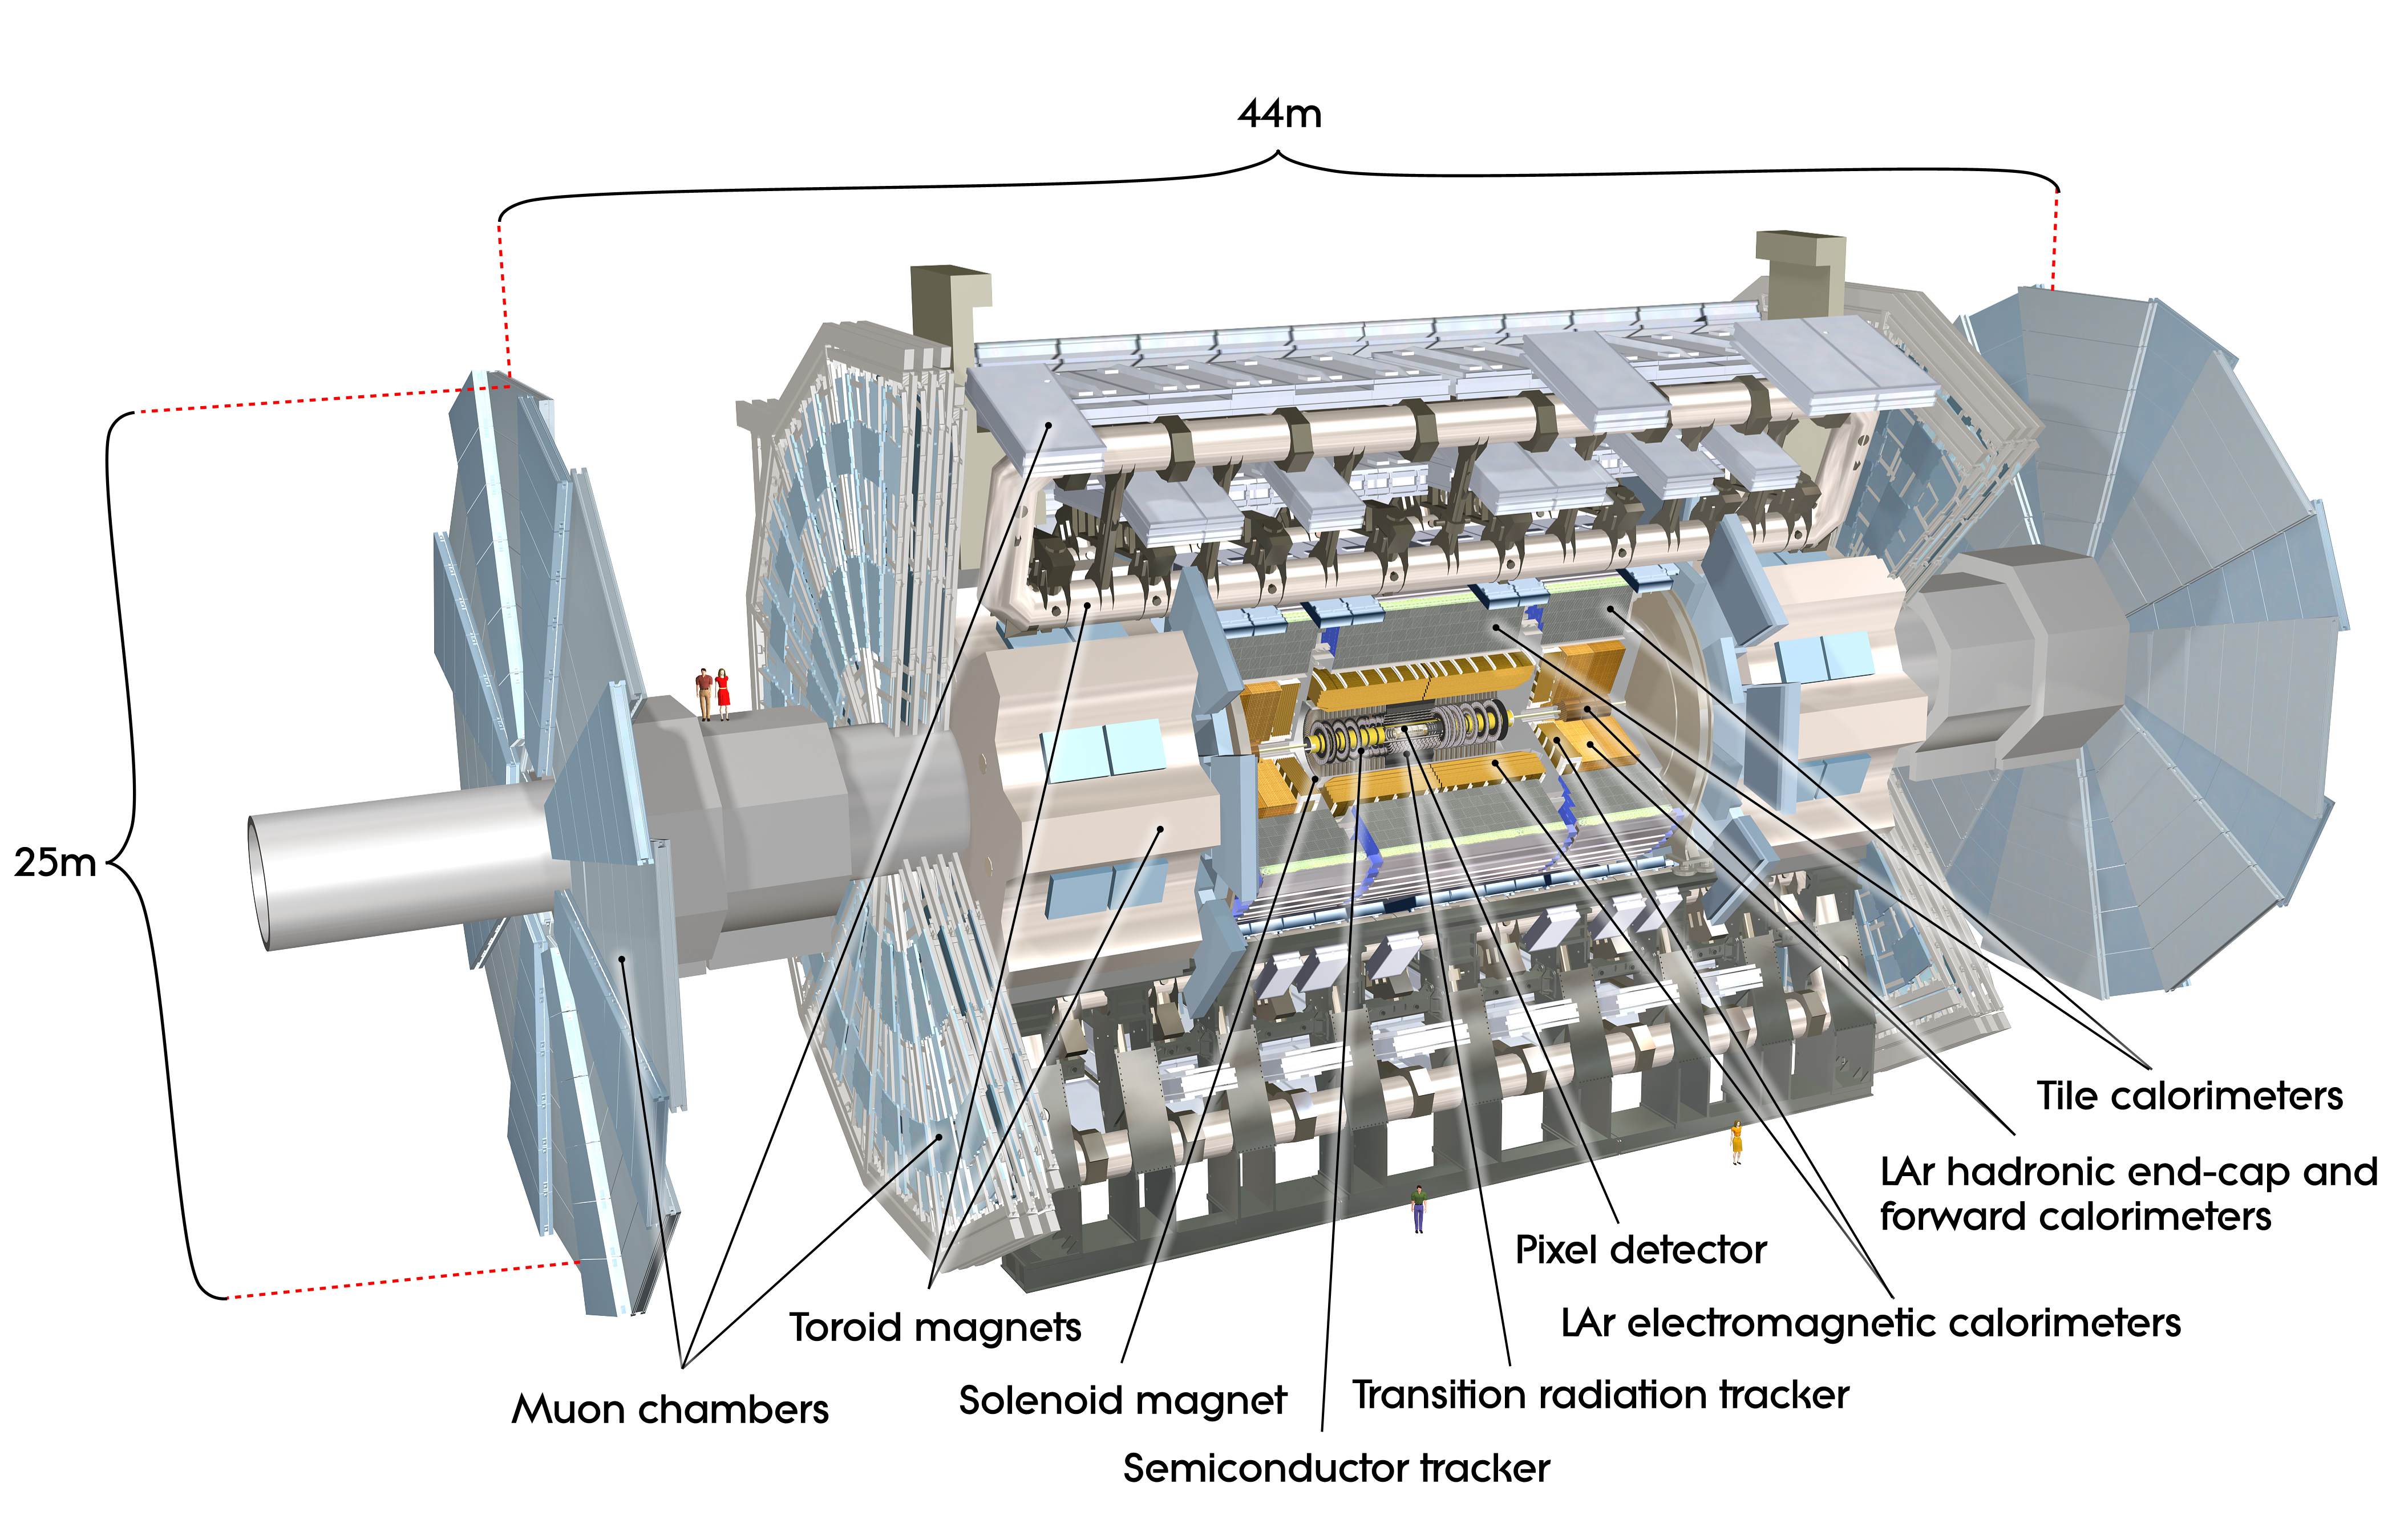
\includegraphics[clip,width=14cm]{fig/2/0803012_01.jpg}
  \caption{ATLAS検出器の全体図}
  \label{fig:ATLAS検出器}
\end{figure}

\subsection{ATLAS検出器における座標系}
ATLAS実験では図\ref{fig:a}に示すような直行座標系と円筒座標系が使用されている。直行座標系では、検出器の中心を原点として、ビーム軸に沿ってz軸を取る。ビーム軸に垂直な平面をx-y平面としたときに、加速器の中心方向を正とするx軸及び、地面に対して垂直方向上向きを正とするy軸を設定する。円筒座標系では、ビーム軸に沿ったz軸に対し、動径方向を$R$、ビーム軸周りの角度を方位角$\phi$、ビーム軸からの角度を極角$\theta$としている。
ATLAS 検出器では z 軸が正の側を A-side、負の側を C-side と定義している。

また、ATLAS実験で使用される座標系として、
\begin{equation}
 \eta=-ln(tan\frac{\theta}{2})
 \label{ラピディティ}
\end{equation}
と定義される擬ラピディティ$\eta$が用いられる。

ATLAS 検出器は円筒形をしており、側面部分と底面部分に配置される検出器を分けて考えるため、$|\eta| < 1.0$ の側面部分をバレル領域、$|\eta| > 1.0$ の底面部分をエンドキャップ領域と呼ぶ。

\begin{figure}[tb]
  \centering
  \includegraphics[clip, width=11cm]{fig/2/atlas_coordinate_fix.pdf}
  \caption{ATLAS検出器における座標系}
  \label{fig:a}
\end{figure}

\subsection{マグネットシステム}\label{magnetic_filed}
ATLAS 実験では、荷電粒子の運動量測定のために超伝導磁石を用いて磁場をかけている。超伝導磁石は 2 種類あり、1 つは衝突点付近で発生した荷電粒子の運動量測定のために用いられるソレノイド磁石、もう 1 つはミューオンの運動量測定のために用いられるトロイド磁石である。
図\ref{fig:磁石}に ATLAS 検出器に設置されている超電導磁石の配置を示す。
トロイド磁石はバレル部とエンドキャップ部に分けられ、それぞれ$\phi$ 方向に 8 つずつ等間隔で配置されている。
トロイド磁石によって生じる磁場の $\eta$ 分布を図\ref{fig:磁場eta}に、x − y 平面での磁場の分布を図\ref{fig:磁場平面} に示す。

\begin{figure}[tb]
  \centering
  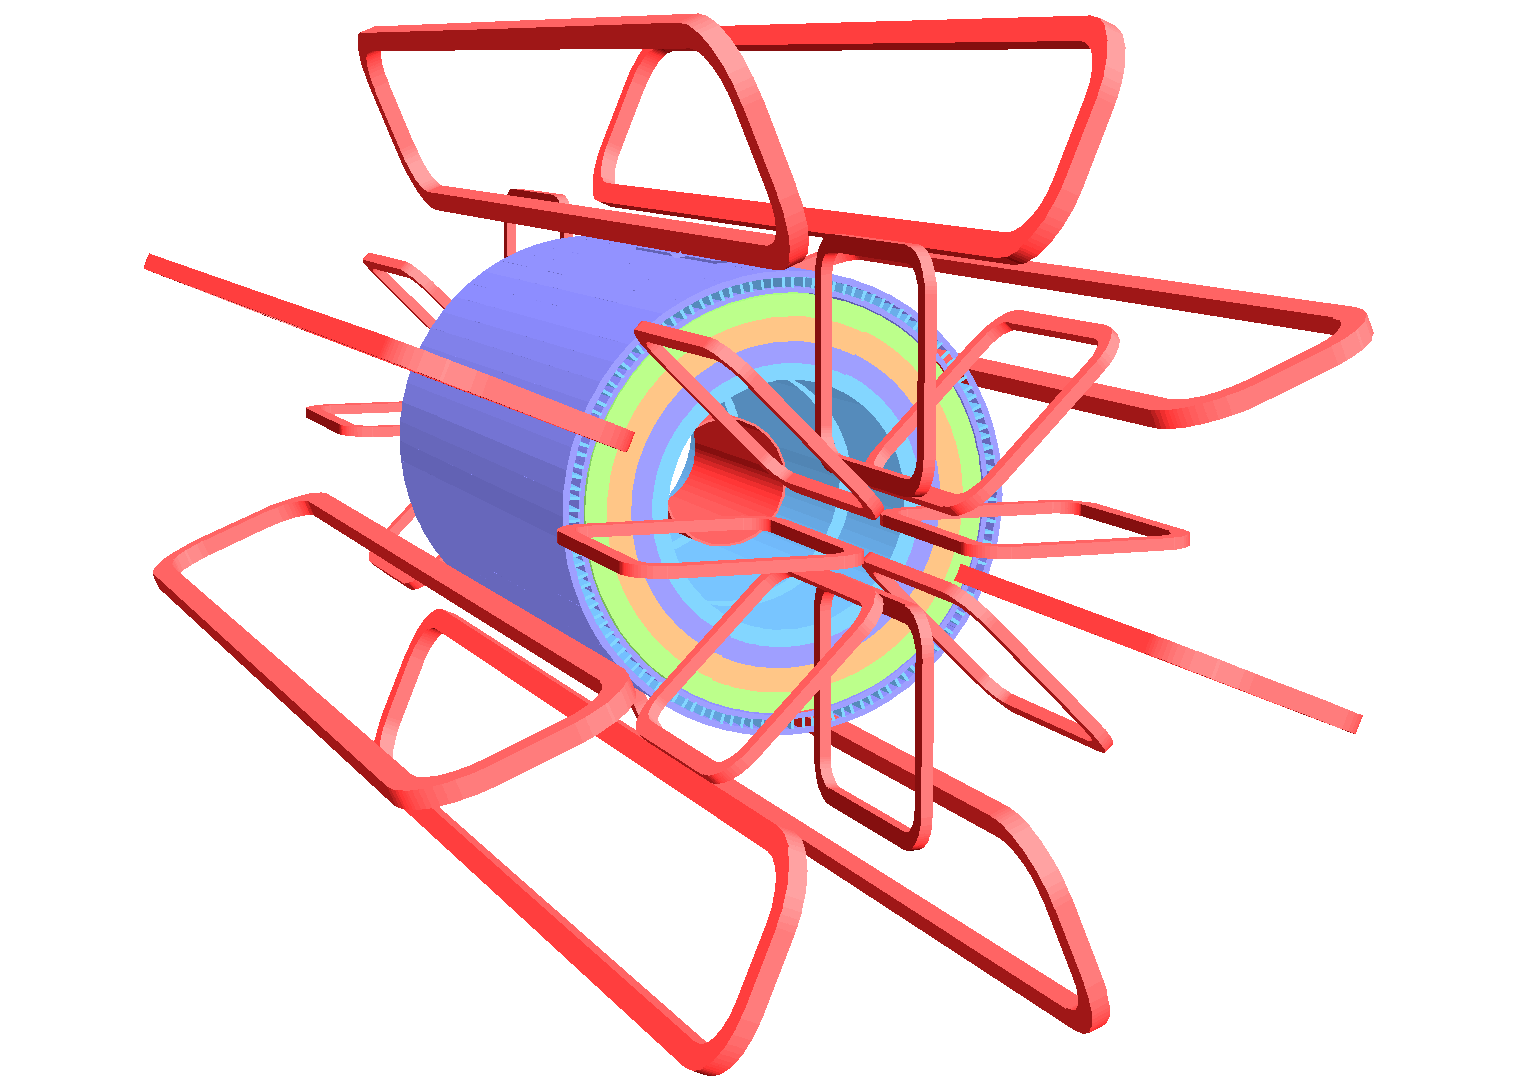
\includegraphics[clip, width=14cm]{fig/2/ATLcoilGeom.pdf}
  \caption{ATLAS検出器で用いられる超電導磁石の配置}
  \label{fig:磁石}
\end{figure}

\begin{figure}
    \centering
    \begin{minipage}[b]{0.4\linewidth}
        \centering
        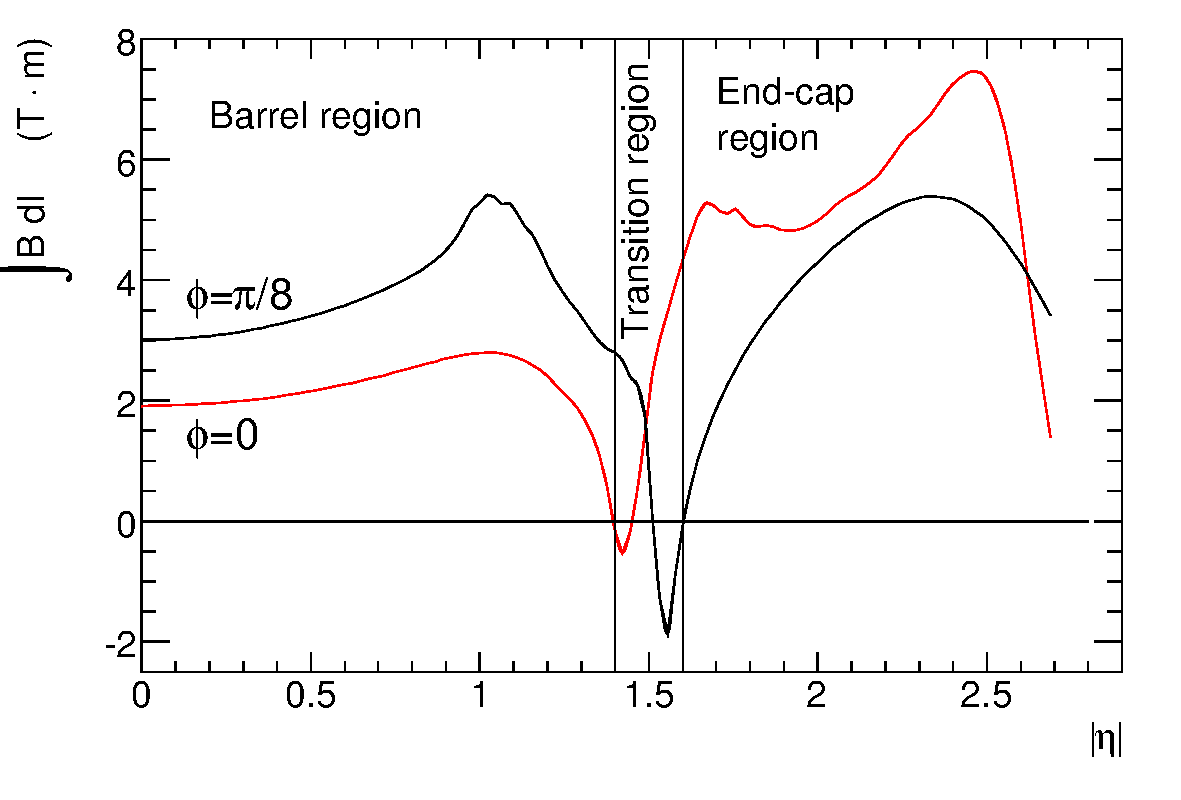
\includegraphics[clip, width=7cm]{fig/2/IBdl.pdf}
        \vspace{10pt}
        \subcaption{}
        \label{fig:磁場eta}
    \end{minipage}
    \hfill
    \begin{minipage}[b]{0.5\linewidth}
        \centering
        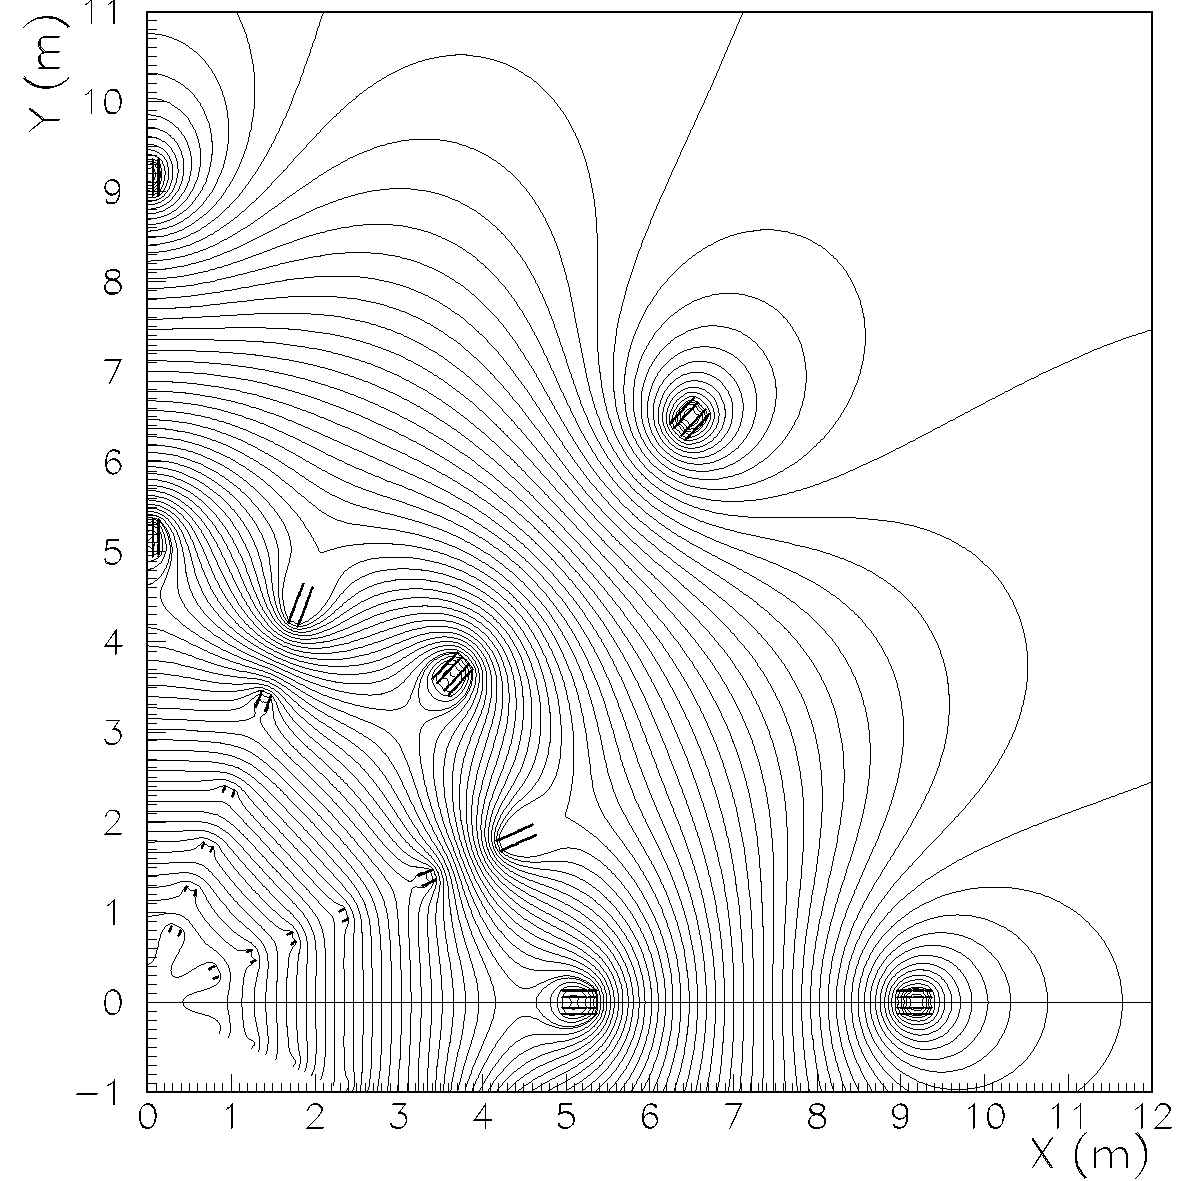
\includegraphics[clip, width=6cm]{fig/2/FMBmap.pdf}
        \vspace{10pt}
        \subcaption{}
        \label{fig:磁場平面}
    \end{minipage}
    \caption{トロイド磁石による磁場の$\eta$分布(a)とビーム軸から見た $x − y$ 平面での磁場の分布(b)。磁石の設置位置の影響により磁場構造が一様ではない。}
    \label{fig:磁場}
\end{figure}




\subsection{内部飛跡検出器}
内部飛跡検出器はビーム衝突点に最も近い位置に設置され、衝突点で発生した荷電粒子の飛跡を測定する。内部飛跡検出器は内側からピクセル検出器 (Pixel)、Semiconductor Tracker (SCT)、Transition Radiation Tracker (TRT) で構成されている。

Pixel は最内層にある半導体検出器であり、高い位置分解能を持つ。
SCT はマイクロストリップと呼ばれる細長い有感領域をシリコン上に施した半導体検出器である。そして TRT は半径 4 mm のチューブ型検出器であり、飛跡のトラッキングのほかに遷移輻射を利用した電子の同定も行っている。図\ref{fig:内部飛跡検出器} に内部飛跡検出器の概略図を示す。

\begin{figure}
    \centering
    \begin{minipage}[b]{0.4\linewidth}
        \centering
        \includegraphics[clip, width=7cm]{fig/2/inner_detectoer1.jpg}
        \vspace{10pt}
        \subcaption{}
        \label{fig:内部飛跡検出器の概略図1}
    \end{minipage}
    \hfill
    \begin{minipage}[b]{0.5\linewidth}
        \centering
        \includegraphics[clip, width=6cm]{fig/2/inner_detector2.jpg}
        \vspace{10pt}
        \subcaption{}
        \label{fig:内部飛跡検出器の概略図2}
    \end{minipage}
    \caption{内部飛跡検出器の全体像及び断面図。(a): 全体像、(b): バレル部の断面図。内側から順に Pixel, SCT, TRT 検出器が設置されている。}
    \label{fig:内部飛跡検出器}
\end{figure}



\subsection{カロリメータ}
カロリメータは、内部飛跡検出器の外側に設置されており、LHCでの陽子衝突で生成された粒子のエネルギー及び位置を測定する役割を担っている。
図\ref{fig:カロリメータ}にATLAS検出器で用いられるカロリメータの概略図を示す。
ATLAS検出器に設置されているカロリメータは、吸収層と検出層からなるサンプリングカロリメータであり、高密度物質の吸収層で粒子シャワーを起こし、検出層で電気信号に変えることで粒子の同定を行っている。
ATLASのカロリメータは、電磁カロリメータとハドロンカロリメータの2種類設置されている。

\begin{figure}[tb]
  \centering
  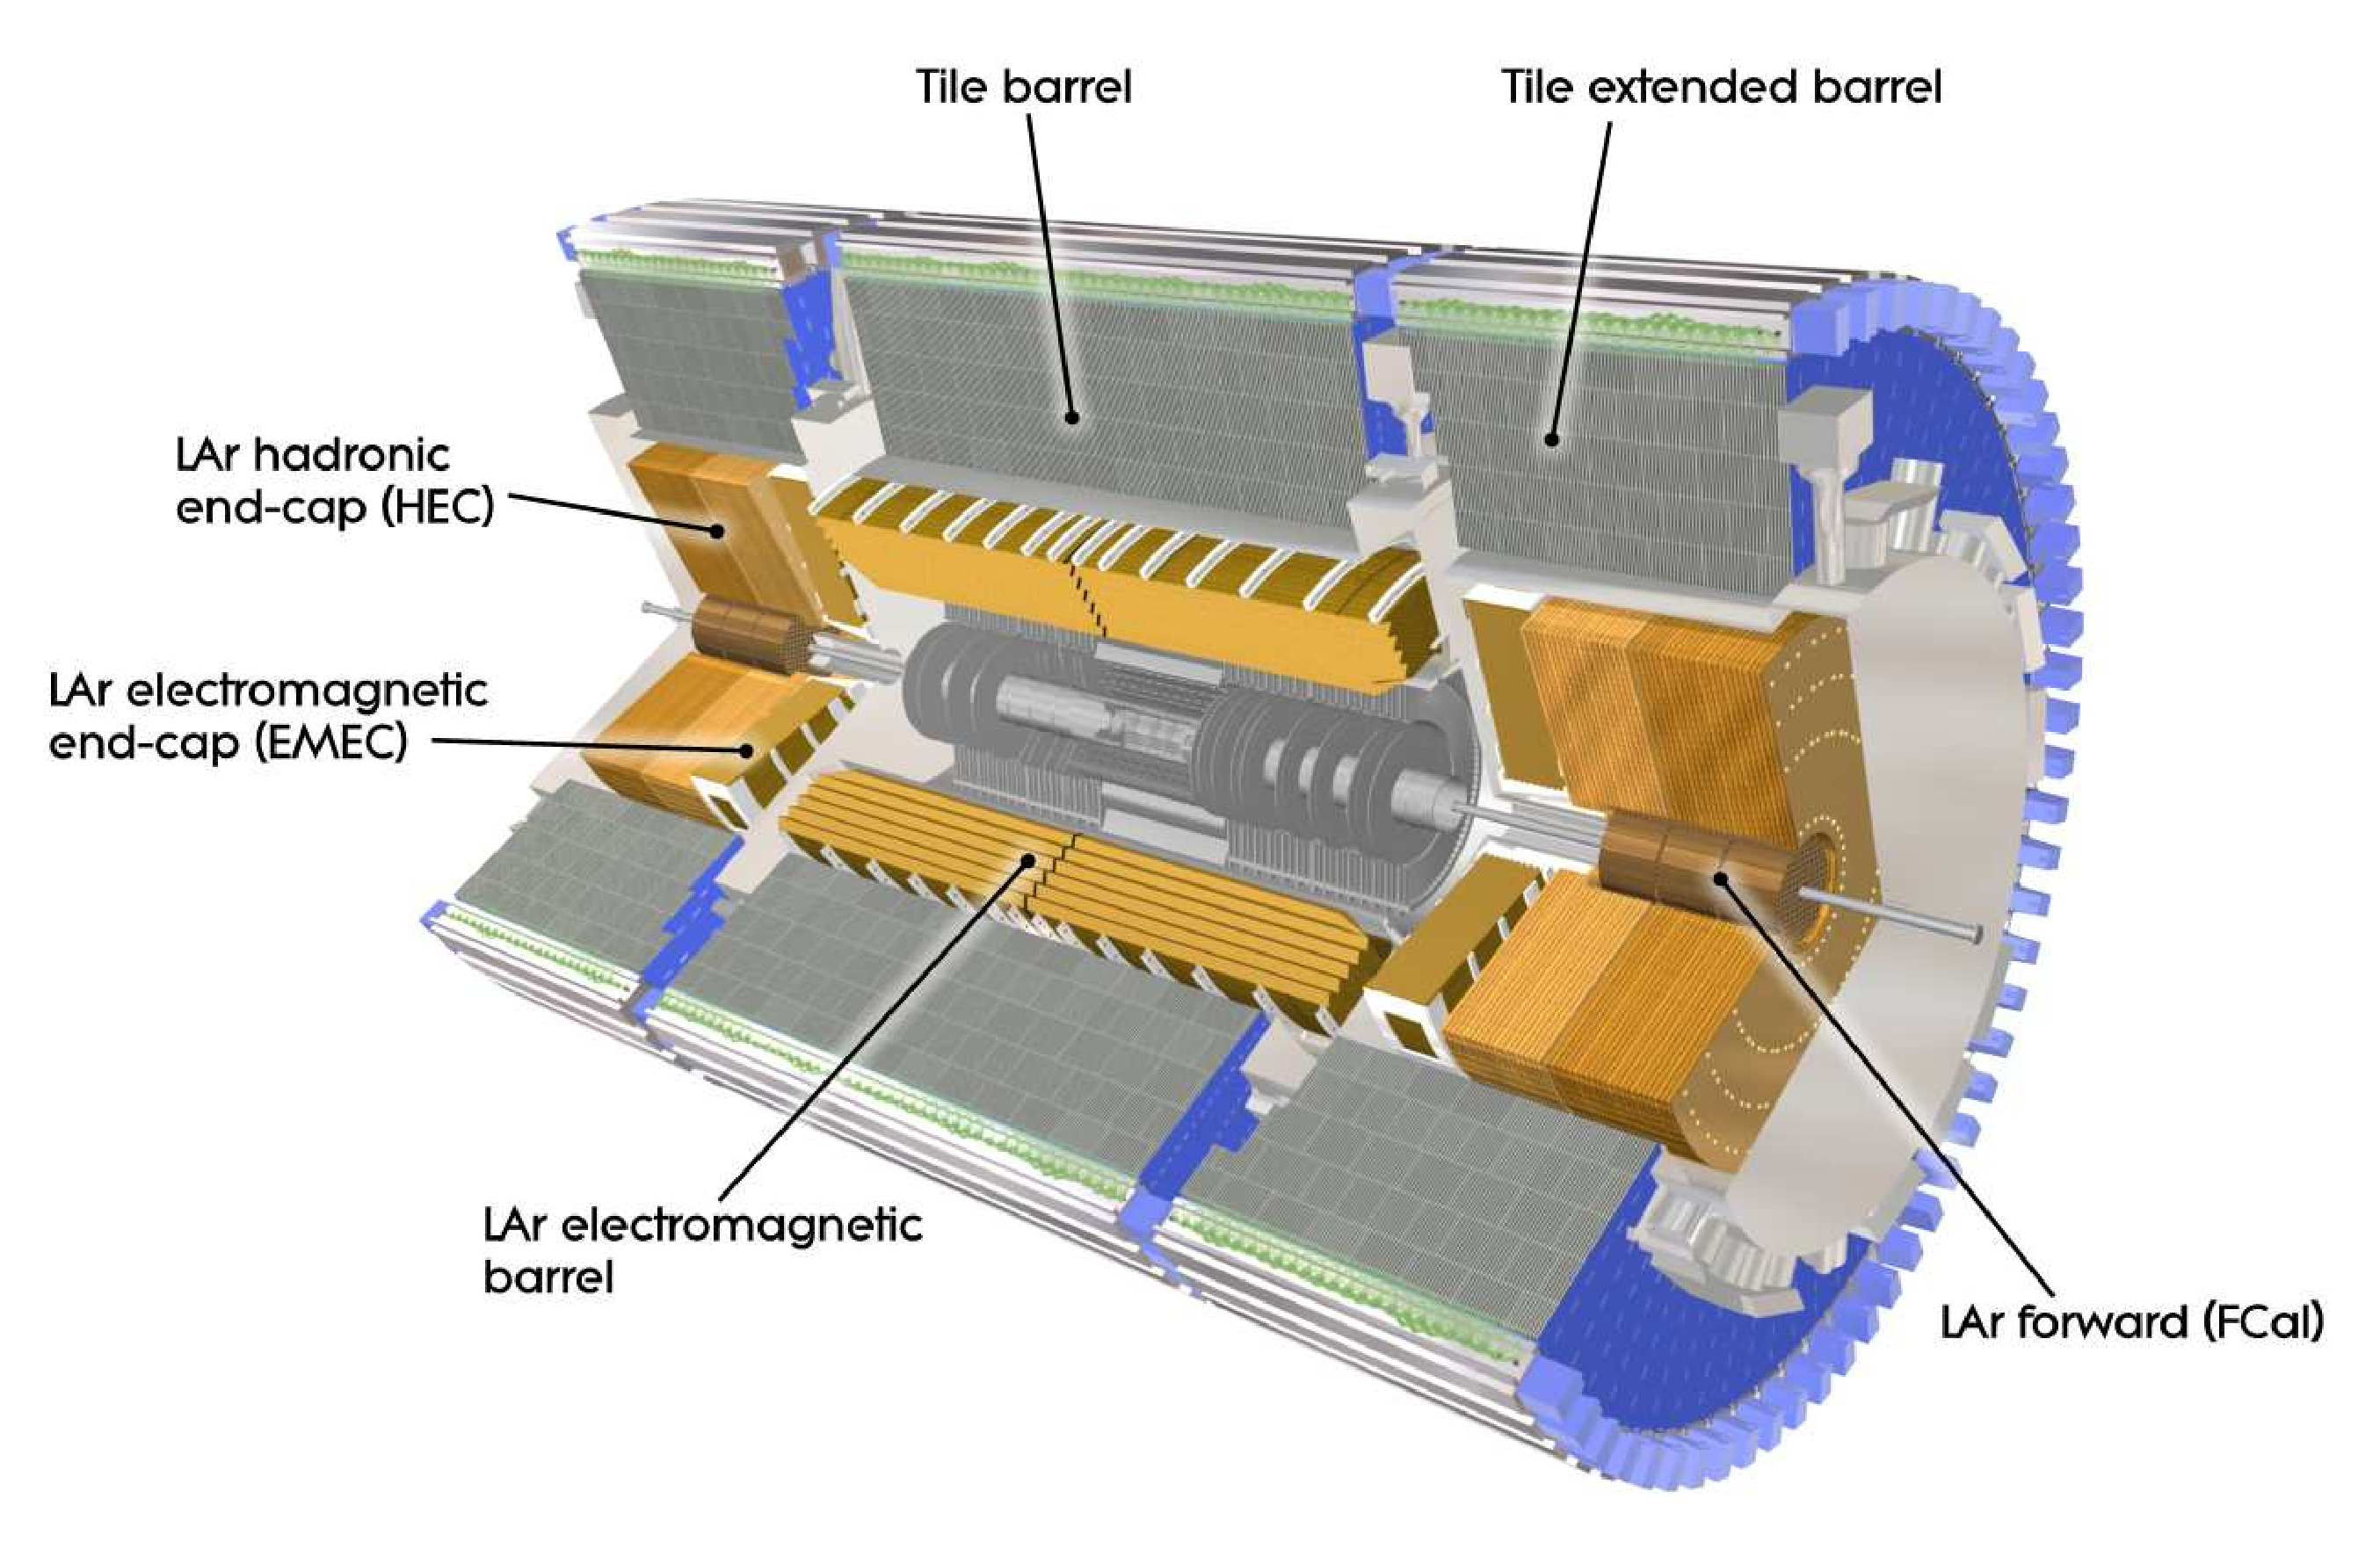
\includegraphics[clip, width=11cm]{fig/2/Calorimeter_d3.pdf}
  \caption{ATLAS 検出器におけるカロリメータの構成。電磁カロリメータは、バレル領域およびエンドキャップ領域の 2 種類。ハドロンカロリメータは、バレル領域のタイル、エンドキャップ領域、フォワード領域の液体アルゴンカロリメータの 3 種類。}
  \label{fig:カロリメータ}
\end{figure}

\subsubsection{電磁カロリメータ}
電磁カロリーメーターは、$|\eta|<1.5$をカバーするバレルカロリメータと、$1.4<|\eta|<3.4$をカバーするエンドキャプカロリメータに分かれている。
バレル部とエンドキャプ部ともに、吸収層の鉛と検出層の液体アルゴンで構成されたカロリメータであり、電磁相互作用を起こす光子や電子のエネルギーと位置を測定する役割を担っている。

\subsubsection{ハドロンカロリメータ}
ハドロンカロリメータは電磁カロリメータの外側に設置されており、タイルカロリーメータ、エンドキャップカロリーメータ、フォワードカロリーメータの3つに分類され、それぞれ異なる$\eta$の範囲をカバーする。バレル部では、鉄の吸収体とタイル状のシンチレータから構成されたタイルカロリメータが設置されている。エンドキャプ部では、銅の吸収体と液体アルゴンから構成されたエンドキャプカロリメータが使用されている。さらに、フォワード領域では銅とタングステンの吸収体と液体アルゴンからなるフォワードカロリメータが設置されている。

\subsection{ミューオン検出器}\label{section2-2-4}
ミューオン検出器は ATLAS 検出器の最外層に設置されており、カロリメータを通過したミューオンを検出するために用いられる。
ミューオン検出器は Resistive Plate Chamber (RPC) と Thin Gap Chamber (TGC) という 2 種類のトリガー検出器と、Monitored Drift Tube (MDT) と Cathode Strip Chamber (CSC) の 2 種類の精密測定用の検出器によって構成される。
図\ref{fig:ミューオン} にミューオン検出器の配置図を示す。

\begin{figure}[tb]
  \centering
  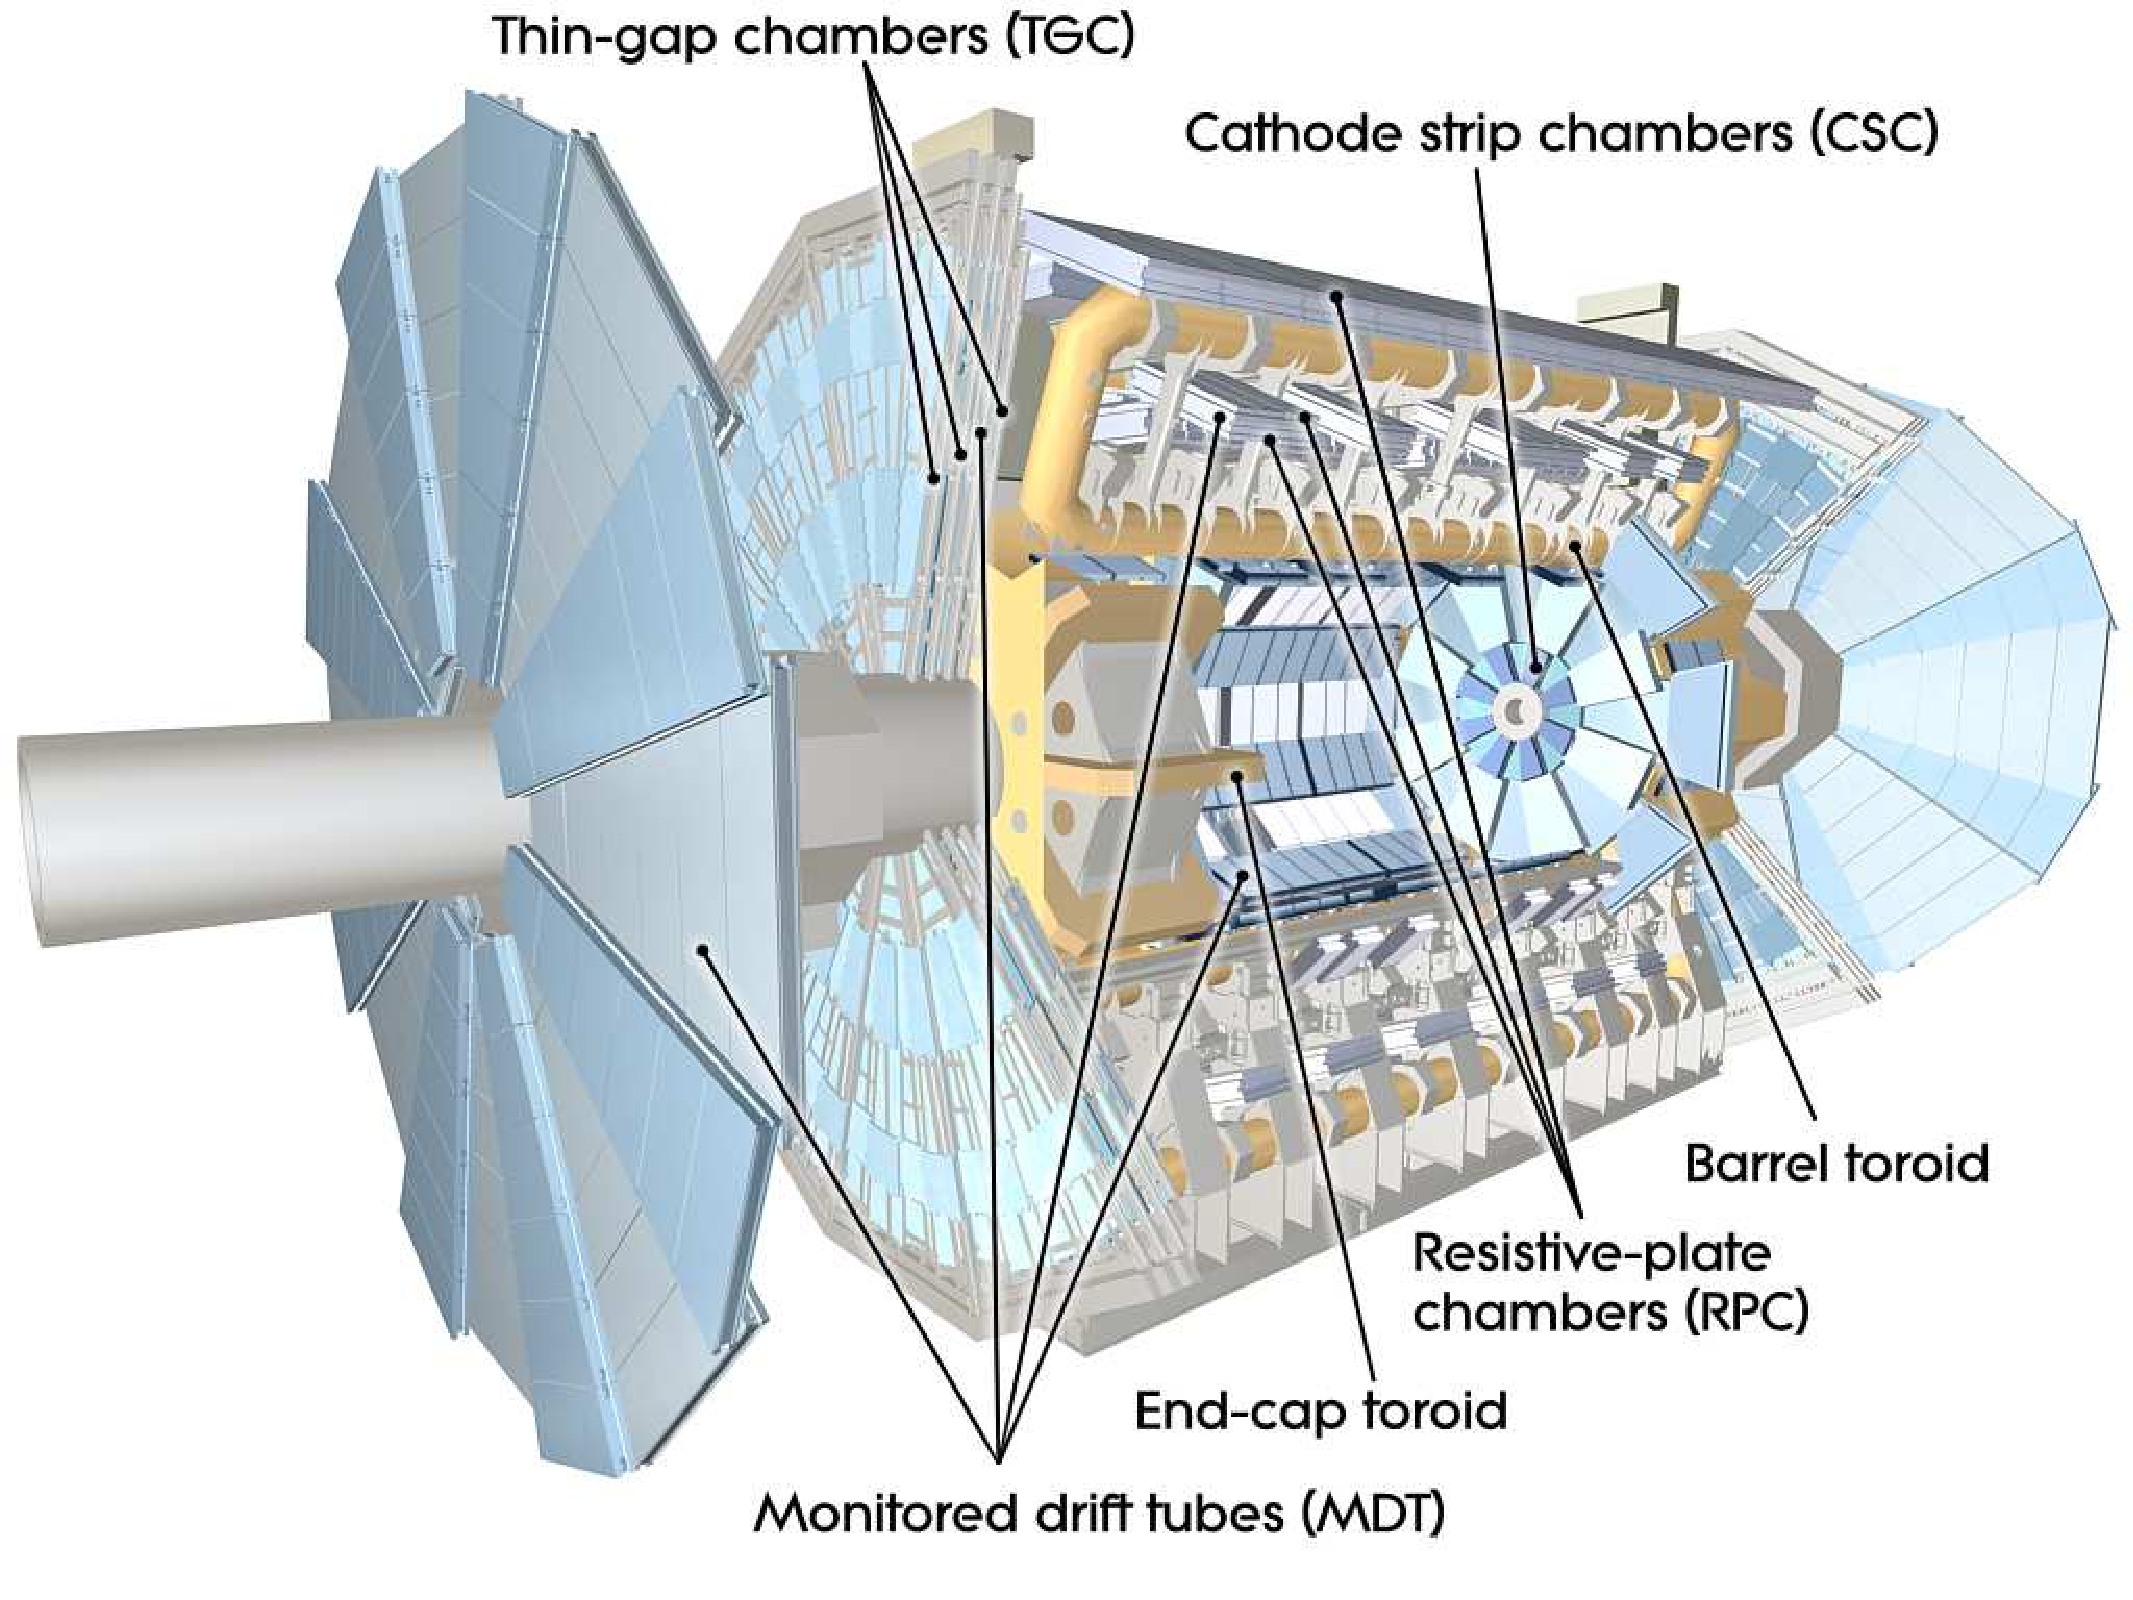
\includegraphics[clip, width=11cm]{fig/2/MuonSystem_d3.pdf}
  \caption{ミューオンスペクトロメータ}
  \label{fig:ミューオン}
\end{figure}

\subsubsection{Resisitive Plate Chamber (RPC)}
RPC はバレル部のミューオントリガー判定に用いられるミューオン検出器である。図\ref{fig:RPC} に RPC 検出器の構造を示す。2 枚の高抵抗プレートの間に幅 2 mm の絶縁体を挟み込んでおり、9.8 kV の高電圧をかけている。各検出器は 2 層構造になっており、直交するストリップの情報から η と φ の位置を読み出している。

\begin{figure}[tb]
  \centering
  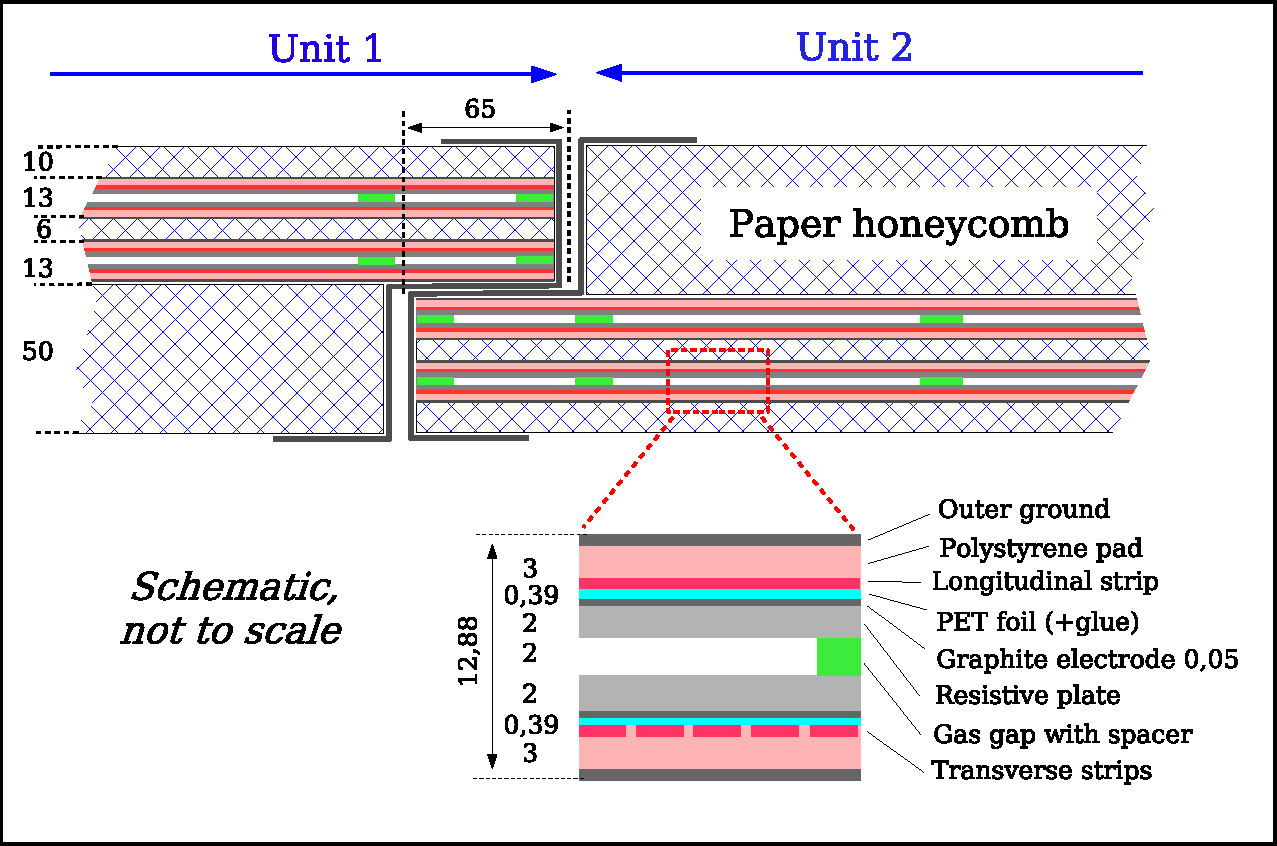
\includegraphics[clip, width=11cm]{fig/2/RPC_structure.pdf}
  \caption{RPCの構造図}
  \label{fig:RPC}
\end{figure}

\subsubsection{Thin Gap Chambers (TGC)}
TGC はエンドキャプ部に設置されているミューオン検出器である。図\ref{fig:TGC_st}にTGC検出器の配置図を示す。TGC検出器はトロイド磁石による磁場領域より内側に EI (Endcap Inner)、FI (Forward Inner)  と呼ばれる 2 つのステーション、磁場領域より外側に M1、M2、M3 (Middle 1,2,3) と呼ばれる 3 つのサブステーションが配置されている。
図\ref{fig:TGC}に示すように、磁場領域より外側にある M1 ステーションは TGC Triplet と呼ばれる3層構造であり、M2、M3 ステーションは TGC Doublet と呼ばれる2層構造である。
M1、M2、M3 は図\ref{fig:TGC_oc} のように円盤状にを配置しており、3 つのステーションを合わせて TGC Big Wheel (TGC BW) と呼ぶ。
M1、M2、M3 からのヒット情報をトリガー判定に使用し、M3 はミューオントリガーの位置情報を決定するための基準として用いられているため、Pivot plane と呼ばれている。
磁場領域より内側にある EI ステーションは TGC Doublet で構成されており、EI チェンバーはトロイド磁石と干渉しないように配置されている。

\begin{figure}[tb]
  \centering
  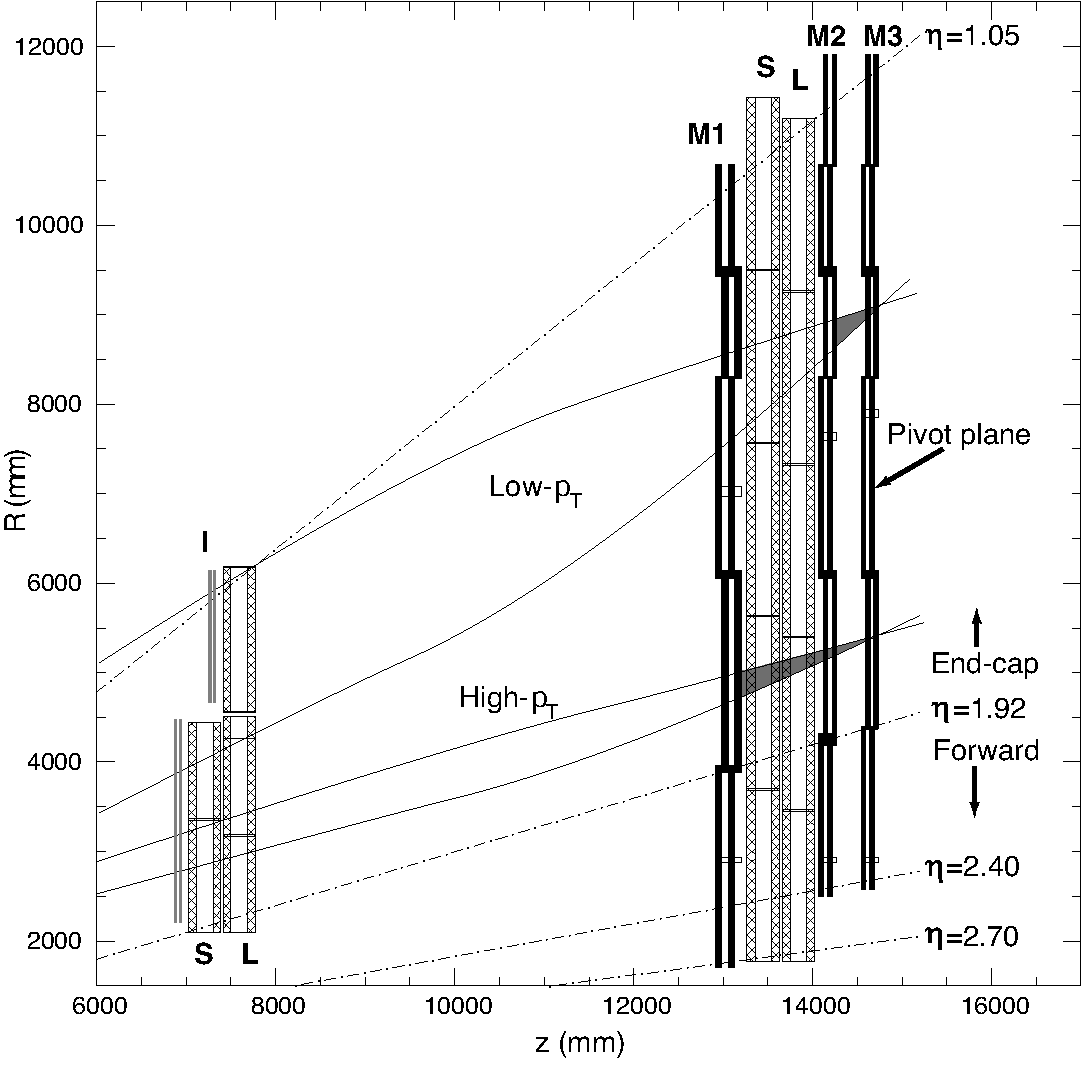
\includegraphics[clip, width=11cm]{fig/2/l1mue-schema.pdf}
  \caption{TGC 検出器の配置図。磁場領域の内側に EI,FI 、外側に M1,M2,M3 が設置されている。}
  \label{fig:TGC_st}
\end{figure}

\begin{figure}[tb]
  \centering
  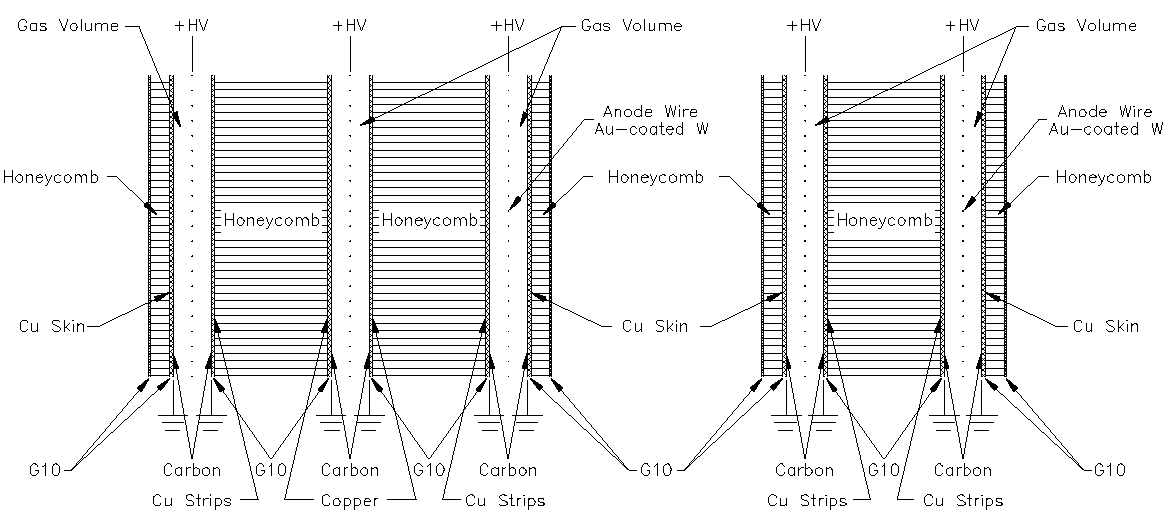
\includegraphics[clip, width=11cm]{fig/2/TGC_construction.pdf}
  \caption{TGC Triplet と Doublet の断面図}
  \label{fig:TGC}
\end{figure}

\begin{figure}[tb]
  \centering
  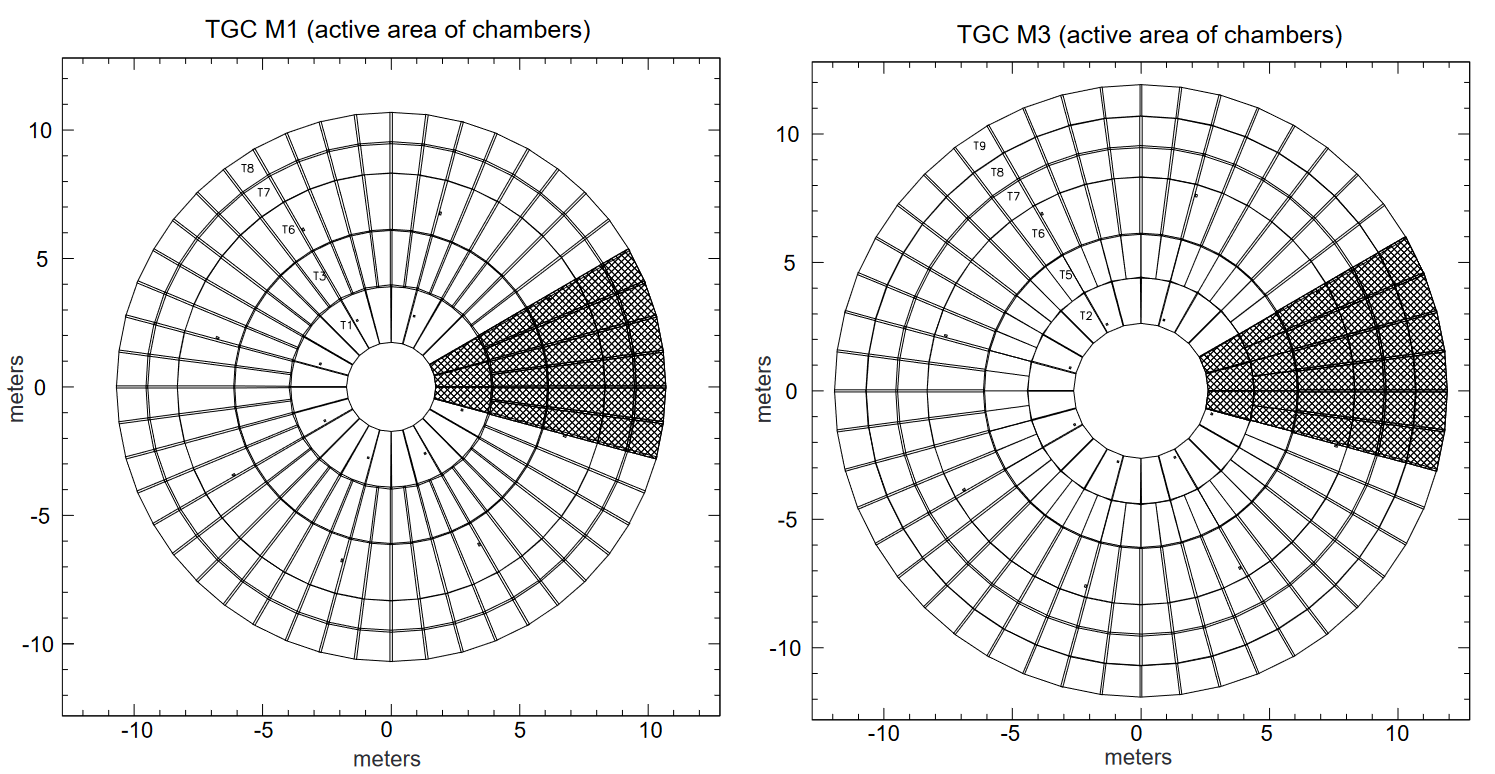
\includegraphics[clip, width=11cm]{fig/2/TGC_octant.png}
  \caption{TGC 検出器 の M1、M3 ステーションの概要図。実線で囲まれたマスが 1 つのチェンバーに対応する。}
  \label{fig:TGC_oc}
\end{figure}

\subsubsection{Monitored Drift Tube (MDT)}
MDT はミューオンの飛跡の精密測定を目的とした検出器であり、直径約 30 mm のドリフトチューブを 6 層または 8 層並べた構造をしている。MDT の構造図を図\ref{fig:MDT} に示す。ドリフトチューブにはアルゴン・二酸化炭素混合ガスを封入している。電離によって生じた電子は、ドリフトチューブの中心に張られている直径 50 $\mu$m のアノードワイヤーで集められる。


\begin{figure}[tb]
  \centering
  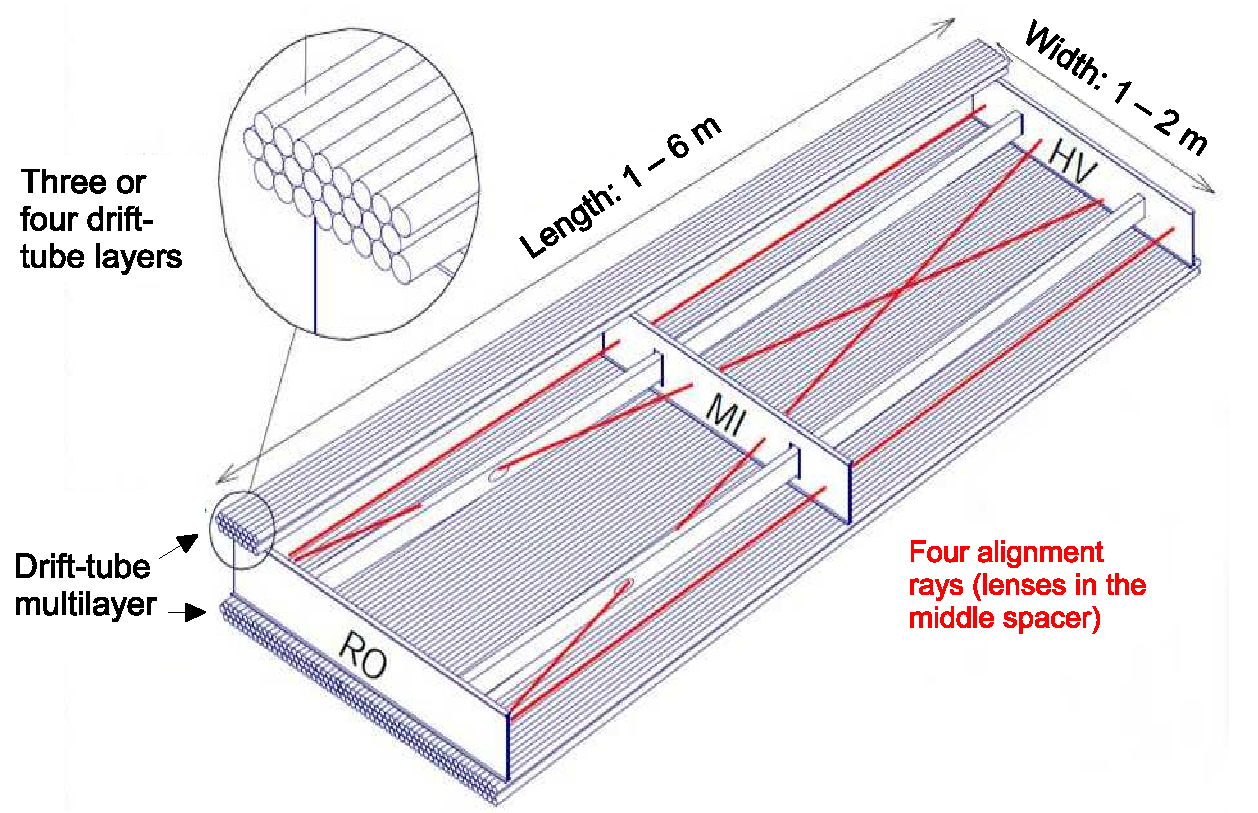
\includegraphics[clip, width=11cm]{fig/2/MDT_chamber_schematics_2.pdf}
  \caption{MDT の構造図}
  \label{fig:MDT}
\end{figure}


\subsubsection{New Small Wheel (NSW)}
New Small Wheel (NSW) は高ヒットレート環境での飛跡測定効率の向上とミューオントリガーの改良を目的として、エンドキャップ部の磁場領域より内側に Run-3 から導入された検出器である。図\ref{fig:NSW}に NSW の全体像を示す。
NSW はエンドキャプ領域の $1.3 < |\eta| < 2.7$ の全$\phi$ 領域を覆うように設置されており、small-strip TGC (sTGC) と Micromegas (MM) の 2 種類の検出器を 4 層ずつ組み合わせた構造をしている。このため、NSW からは位置情報だけでなく飛跡の再構成による角度情報も得ることができる。

\begin{figure}[tb]
  \centering
  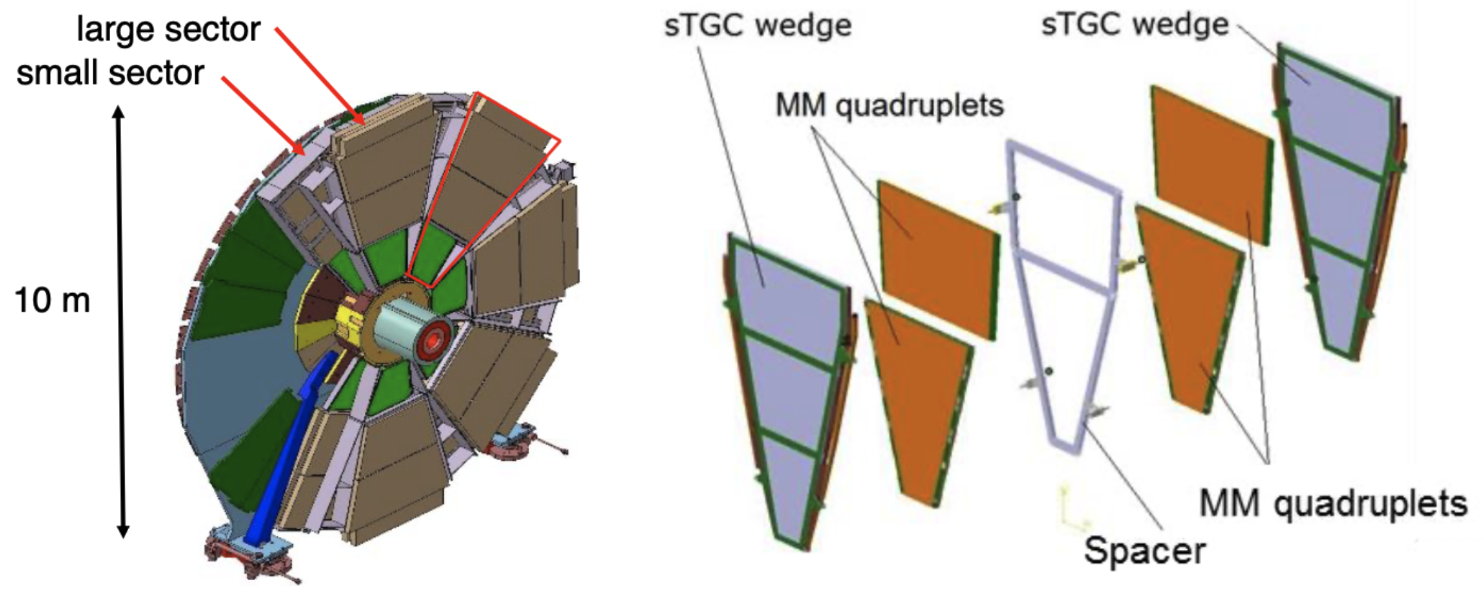
\includegraphics[clip, width=11cm]{fig/2/nsw-structure.png}
  \caption{NSW の構造。Large Sector と Small Sector の 2 種類のチェンバーを交互に配置している。sTGC quadruplet の間に、4 層で構成されている MM が 2 つ挟まれており、合計 16 層で構成されている。}
  \label{fig:NSW}
\end{figure}

\subsubsection{small-strip TGC (sTGC)}
small-strip TGC (sTGC) は TGC と同様の 2.8 mm のガスギャップを持つ MWPC である。図\ref{fig:sTGC}に示すように sTGC は TGC と異なり、ストリップを用いて η 方向の位置座標を、ワイヤーを用いて φ 方向の位置座標を測定する。sTGC にはパッドと呼ばれる読み出しカソードがあり、ストリップとパッドでアノードワイヤーを挟む構造になっている。パッドは長方形の電極であり、まずパッドを用いて大まかな位置情報を計算し信号を読み出す領域を限定する。そして、限定された領域のストリップ情報を用いてより精密な位置情報の計算を行うことで高速な飛跡再構成を行う。

\begin{figure}[tb]
  \centering
  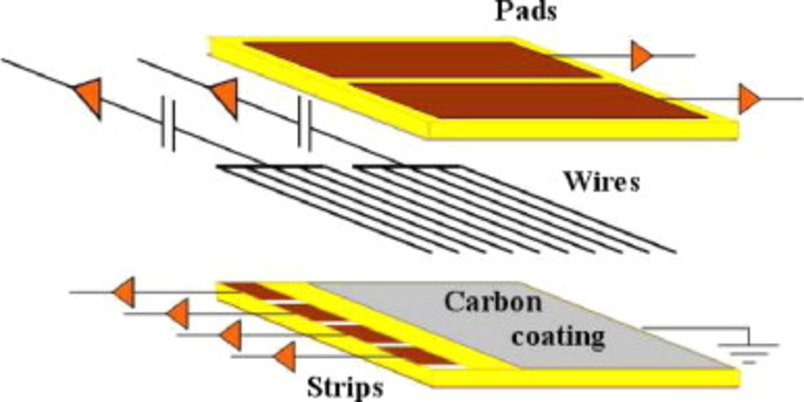
\includegraphics[clip, width=10cm]{fig/2/stgc-structure.pdf}
  \caption{sTGC の断面図。 パッド、ストリップを用いて $\eta$ を、ワイヤーを用いて $\phi$ を計算する。}
  \label{fig:sTGC}
\end{figure}

\subsubsection{Micromegas (MM)}
Micromegas (MM) は、ワイヤーを用いないガス検出器である。図\ref{fig:MM}に MM の概要図を示す。MM は、厚さ 5 mm のドリフト領域と 128 μm の増幅領域がメッシュで隔てられている構造である。増幅領域では電子のみでなく陽イオンも生成されるが、MM では増幅領域の厚さが小さいため、高レート環境でも陽イオンによる影響を抑えることができる。
また、読み出された信号の時間差を用いることで飛跡の z 方向の情報を再構成することができる。これにより位置分解能 90 μm という高い精度での測定が可能である。

\begin{figure}[tb]
  \centering
  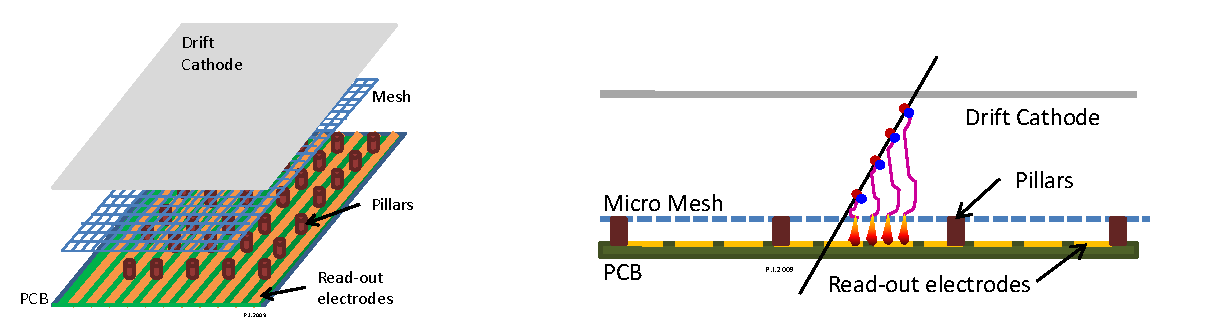
\includegraphics[clip, width=13cm]{fig/2/mm-structure.pdf}
  \caption{MM の概略図。メッシュによってドリフト領域と増幅領域に分けられる。ドリフト領域で生成された電子はメッシュを通過し、増幅領域で形成された電場により増幅される。}
  \label{fig:MM}
\end{figure}








